\documentclass[11pt]{article}
\usepackage{macros}
\usepackage{CJKutf8}
\parindent0in
\pagestyle{plain}
\thispagestyle{plain}

\scribedby{Scribed By: Tao Huang}
\assignment{ShanghaiTech University, China}
\lecturedate{January 10, 2021}

\begin{document}
\begin{CJK*}{UTF8}{gbsn}
\maketitle

\outline{This note dedicates to conclude some important contents of Statistical Learning by Hang Li, augmented by some insights and self-understanding to them. The organization follows directly from Li, and I wish it can help you dive deeper in this interesting area. Let's start now!}\par

%%% Start writing and defining sections and subsections here
\tableofcontents
\clearpage
\section{Introduction to Statistical Learning}

%---------Perceptron---------
\section{Perceptron}
\subsection{Model}
\begin{align*}
	f(x) = sign(w\cdot x +b)
\end{align*}

\begin{align*}
	sign(x)=\left\{
\begin{aligned}
 &   +1, \quad & x\ge 0\\
 &   -1,  \quad & x <0
\end{aligned}
\right.
\end{align*}

\subsection{Strategy}
\begin{align*}
	\min_{w,b} L(w,b) = -\sum_{x\in M} y_i(w\cdot x_i + b)
\end{align*}

\subsection{Algorithm}
\subsubsection{Primal Problem}
\begin{align*}
	w &\leftarrow w + \eta \nabla_w L(w,b) = w + \eta \sum_{x\in M}y_ix_i \\
	b &\leftarrow b + \eta \nabla_b L(w,b) = b + \eta \sum_{x\in M}y_i \\
\end{align*}

\subsubsection{Dual Problem}
\begin{align*}
	w &= \sum_{i=1}^N n_i\eta y_ix_i \triangleq \sum_{i=1}^N \alpha_iy_ix_i\\
	b &= \sum_{i=1}^N \alpha_iy_i
\end{align*}

\begin{align*}
	\alpha_i &\leftarrow \alpha_i + \eta\\
	b &\leftarrow b + \eta y_i
\end{align*}

\subsubsection{Convergence}
\begin{proof}
(1) 
\begin{align*}
	\gamma = \min_{i}\{y_i(\hat{w}_{opt}\cdot \hat{x}_{i})\}
\end{align*}
(2) 
\begin{align*}
	\hat{w}_k \leftarrow \hat{w}_{k-1} + \eta y_i\hat{x}_i
\end{align*}

\begin{align*}
	\hat{w}_k \cdot \hat{w}_{opt} &\ge k\eta\gamma \\
	 \|\hat{w}_k\|^2  &\le k\eta^2R^2
\end{align*}
\end{proof}

%---------KMeans---------
\section{K-Means}

%---------Naive Bayes---------
\section{Naive Bayes}

%---------Decision Tree---------
\section{Decision Tree}

%---------LR MEM---------
\section{LR \& MEM}

%---------SVM---------
\section{Support Vector Machine}

%---------Boosting---------
\section{Boosting}

%---------EM Algorithm---------
\section{EM Algorithm}

\begin{align*}
	\theta^\star = \arg\max_{\theta}\log P(X_1,X_2,...,X_n|\theta)
\end{align*}

\begin{align*}
	\theta^\star = \arg\max_{\theta} P(\theta|X_1,...,X_n) = \arg\max_{\theta}\frac{P(X_1,...,X_n,\theta)}{P(X_1,...,X_n)}
\end{align*}

\begin{align*}
	L(\theta) &= \log P(Y|\theta)\\
					&= \log \sum_Z P(Y,Z|\theta)\\
					&= \log \left(\sum_Z P(Z|Y,\theta)P(Y|\theta)\right)
\end{align*}

\begin{align*}
	L(\theta) - L(\theta^{(i)}) &= \log \sum_Z P(Y,Z|\theta) - \log P(Y|\theta^{(i)})\\
		&= \log  \sum_Z P(Z|Y,\theta^{(i)}) \frac{P(Y,Z|\theta)}{P(Z|Y,\theta^{(i)})} -  \log P(Y|\theta^{(i)})\\
		&\ge \sum_Z P(Z|Y,\theta^{(i)})\log \frac{P(Y,Z|\theta)}{P(Z|Y,\theta^{(i)})} - \log P(Y|\theta^{(i)})\\
		&= \sum_Z P(Z|Y,\theta^{(i)})\log \frac{P(Y,Z|\theta)}{P(Z|Y,\theta^{(i)})} - \sum_Z  P(Z|Y,\theta^{(i)})\log P(Y|\theta^{(i)}) \\
		&= \sum_Z P(Z|Y,\theta^{(i)}) \log \frac{P(Y,Z|\theta) }{P(Z|Y,\theta^{(i)}) P(Y|\theta^{(i)})}
\end{align*}

$$B(\theta,\theta^{(i)}) = L(\theta^{(i)}) + \sum_Z P(Z|Y,\theta^{(i)}) \log \frac{P(Y,Z|\theta) }{P(Z|Y,\theta^{(i)}) P(Y|\theta^{(i)})}$$

\begin{align*}
	\theta^{(i+1)} &= \arg\max_\theta B(\theta, \theta^{(i)})\\
	&= \arg\max_\theta\left( L(\theta^{(i)}) + \sum_Z P(Z|Y,\theta^{(i)}) \log \frac{P(Y,Z|\theta) }{P(Z|Y,\theta^{(i)}) P(Y|\theta^{(i)})}\right)\\
	&= \arg\max_\theta \sum_Z P(Z|Y,\theta^{(i)})  \log P(Y,Z|\theta)\\
	& \triangleq\arg\max_\theta Q(\theta, \theta^{(i)})
\end{align*}

\begin{align*}
	Q(\theta, \theta^{(i)}) &= E_Z\left[\log P(Y,Z|\theta)|Y,\theta^{(i)} \right]\\
	&=\sum_Z P(Z|Y,\theta^{(i)})  \log P(Y,Z|\theta)
\end{align*}

%---------HMM---------
\section{Hidden Markov Model}

% \begin{figure}[h]
%    \centering
%    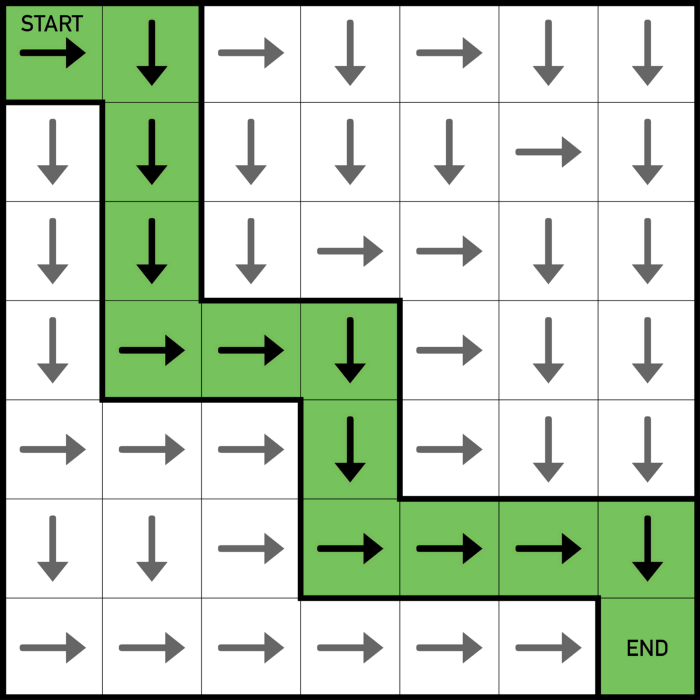
\includegraphics[width=0.5\linewidth]{assets/gridworld.png}
%    \caption{A sample figure depicting a gridworld}
%    \label{figure:gridworld}
% \end{figure}


%Keep figures (\texttt{.eps},\texttt{.jpg/png/etc},\texttt{.pdf}) and source codes inside the \texttt{assets/} folder. Please look at tthe source of Figure \ref{figure:gridworld} for reference.


\bibliographystyle{unsrt}
\bibliography{main}

\end{CJK*}
\end{document}  